\chapter{Evaluation}
\label{evaluation}

\section{Experiment}

The author performed several experiments using QuISP (Quantum Internet Simulation Package) and demonstration of the proposed protocol in several circumstances.

\subsection{Validation of the protocol}
The author ran the simulations whose topology has two nodes with a single link for two different link architectures, which are SenderReceiver and MeetInTheMiddle.

\begin{figure}[H]
  \centerline{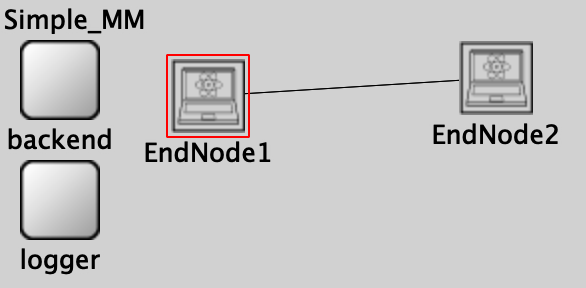
\includegraphics[width=.8\columnwidth]{images/topology_MM.png}}
  \caption{Network topology for SenderReceiver}
\end{figure}

\begin{figure}[H]
  \centerline{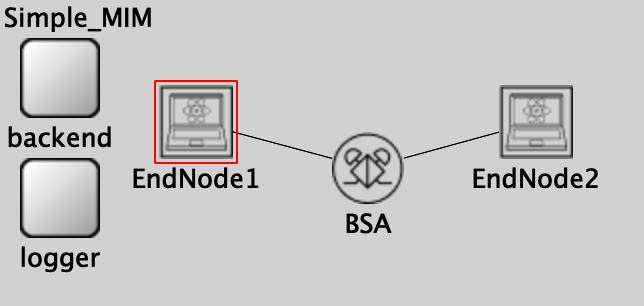
\includegraphics[width=.8\columnwidth]{images/topology_MIM.png}}
  \caption{Network topology for MeetInTheMiddle}
\end{figure}

The active link allocation policy, the next link allocation policy, and the first sequence number for the new allocation policy became coordinated in these two nodes, both before the connection setup and before the connection teardown in both cases,
which means that the proposed link management protocol is independent from the underlying physical link architecture.

\begin{table}[ht]
  \begin{center}
    \begin{tabular}{|m{5em}|m{5em}|m{10em}|m{10em}|m{5em}|} \hline
      Case & Node name  & Active link allocation policy & Next link allocation policy & The sequence number of the first Bell pair \\ \hline \cline{1-5}
      Connection Setup & Node 1 & [] & [7640092079844890364, 5401871878593356085] & 1 \\ \cline{1-5}
       & Node 2 & [] & [7640092079844890364, 5401871878593356085] & 1 \\ \cline{1-5}
       Connection Teardown & Node 1 & [7640092079844890364, 7640092079844890364]& [] & 1 \\ \cline{1-5}
       & Node 2 & [7640092079844890364, 7640092079844890364] & [] & 1 \\ \cline{1-5}
    \end{tabular}
    \caption{A table for the outcome of the negotiation between two nodes in the MM simulation}
  \end{center}
\end{table}

\begin{table}[ht]
  \begin{center}
    \begin{tabular}{|m{5em}|m{5em}|m{10em}|m{10em}|m{5em}|} \hline
      Case & Node name  & Active link allocation policy & Next link allocation policy & The sequence number of the first Bell pair \\ \hline \cline{1-5}
      Connection Setup & Node 1 & [] & [5401871878593356085, 864743034342436556] & 1 \\ \cline{1-5}
       & Node 2 & [] & [5401871878593356085, 864743034342436556] & 1 \\ \cline{1-5}
       Connection Teardown & Node 1 & [7640092079844890364, 7640092079844890364] & [] & 1 \\ \cline{1-5}
       & Node 2 & [7640092079844890364, 7640092079844890364] & [] & 1 \\ \cline{1-5}
    \end{tabular}
    \caption{A table for the outcome of the negotiation between two nodes in the MIM simulation}
  \end{center}
\end{table}

\newpage

\subsection{Ratio of Bell pairs allocated to each connection}

The following figure compares the ratio of the Bell pairs allocated to each Bell pairs. It shows that all the Bell pairs are allocated if there is only a single connection, and half of them are allocated if there are two active connections.

\begin{figure}[H]
  \centerline{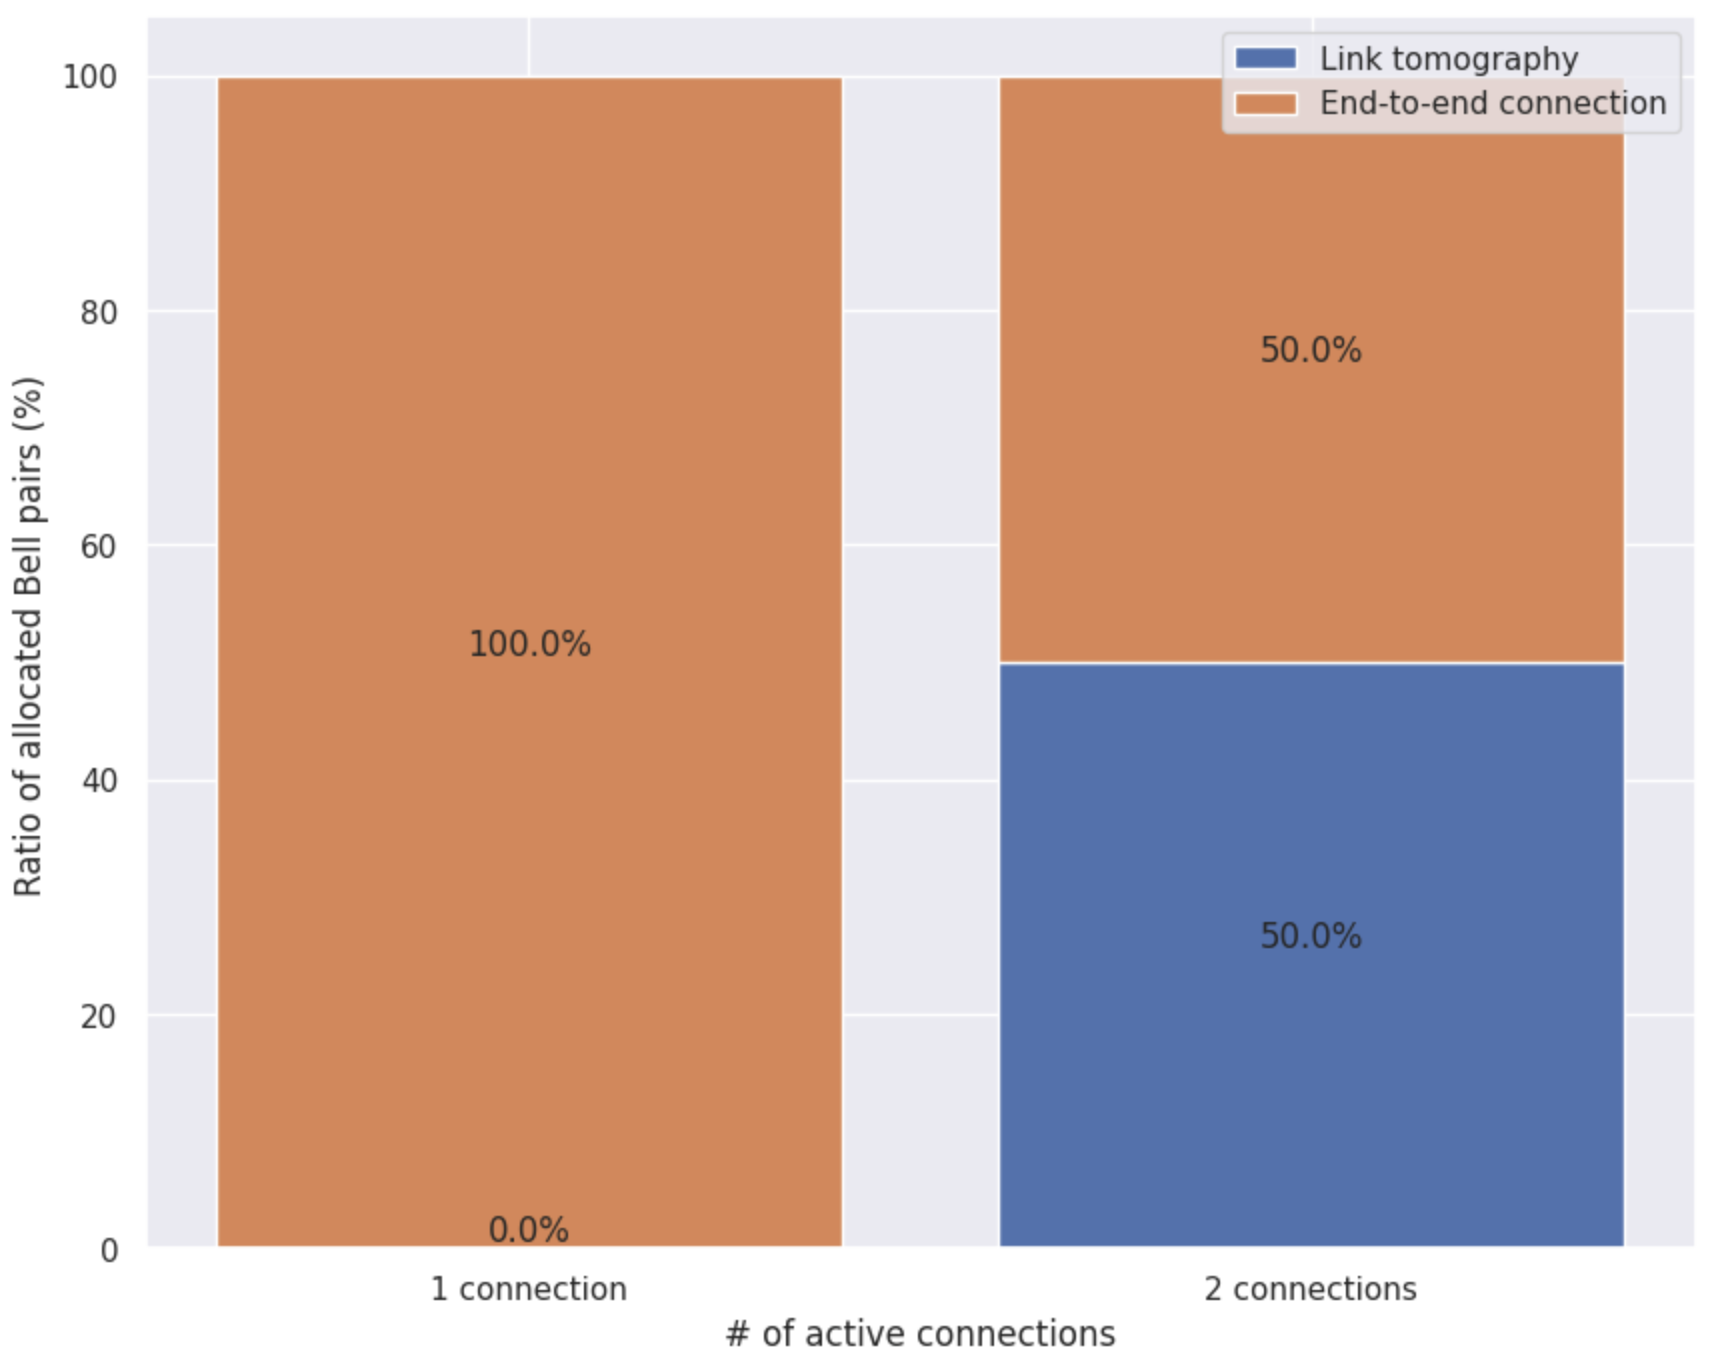
\includegraphics[width=.8\columnwidth]{images/ratio_of_bell_pairs.png}}
  \caption{The figure of the ratio of allocated Bell pairs}
\end{figure}

\subsection{Validation of release of the Bell pairs}

The following figure shows that the number of allocated Bell pairs in the entire network decreases at the end of the simulation.
It demonstrates the fact that the Bell pairs that were allocated to but not consumed by the active connections are successfully released after the teardown of those connections.

\begin{figure}[H]
  \centerline{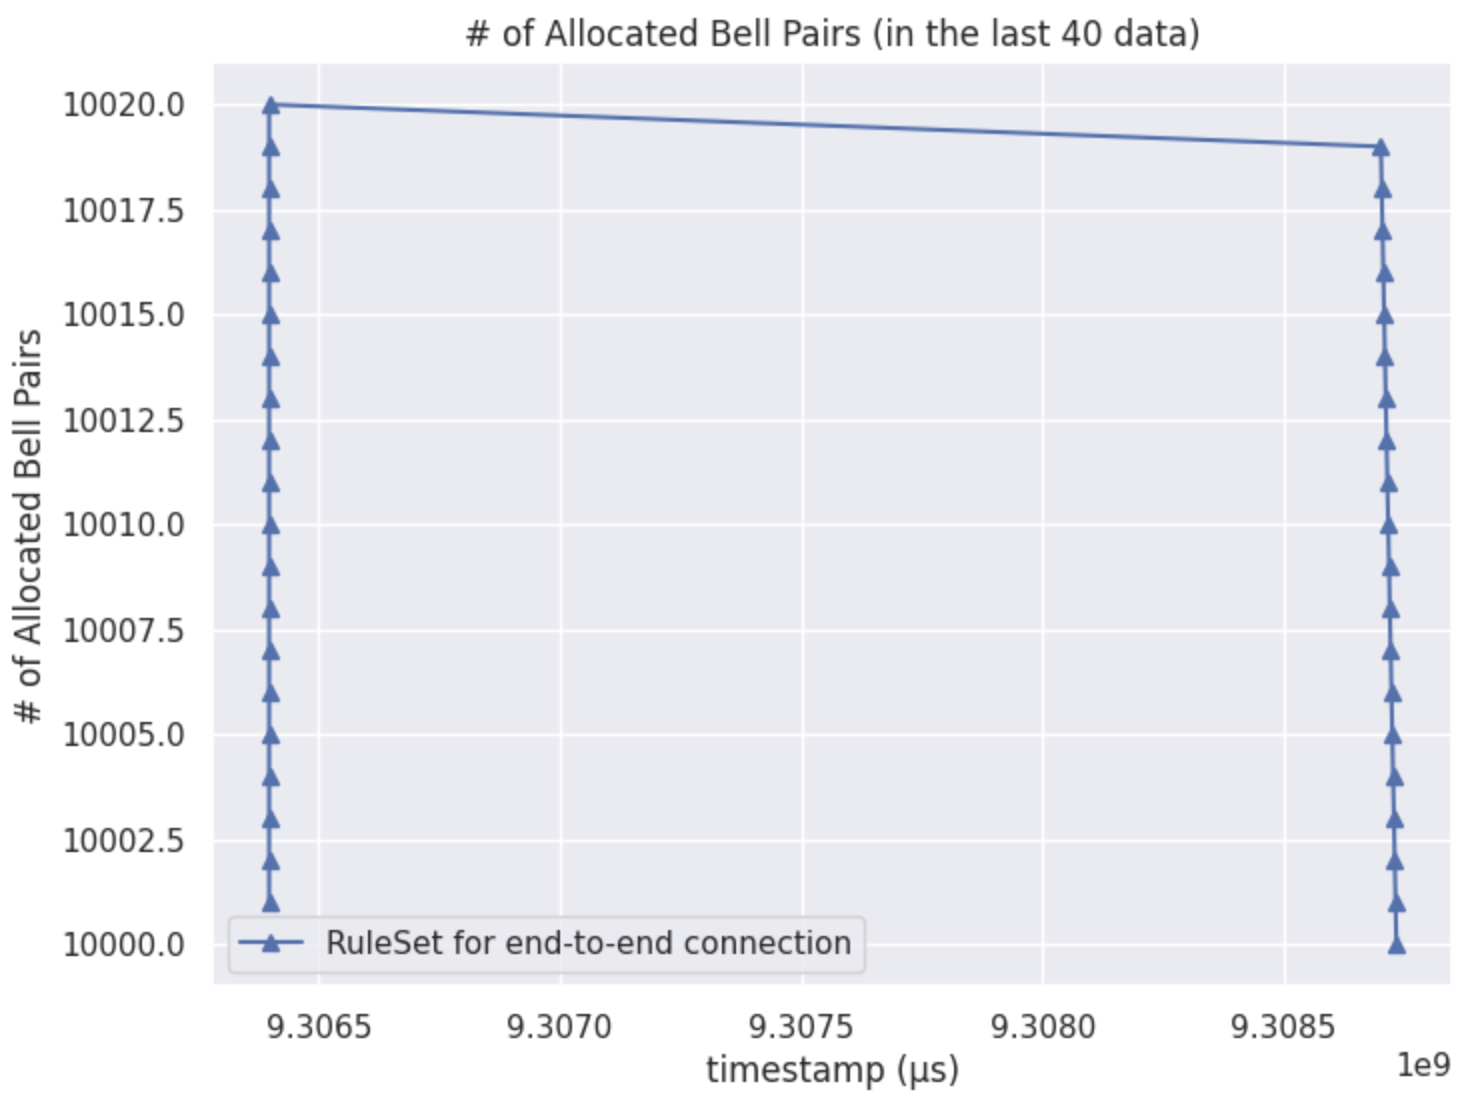
\includegraphics[width=.8\columnwidth]{images/number_of_bell_pairs.png}}
  \caption{The figure of the total number of allocated Bell pairs in the last 40 timestamps}
\end{figure}



%%% Local Variables:
%%% mode: japanese-latex
%%% TeX-master: "./thesis"
%%% End:
